\documentclass{article}
\usepackage{nips15submit_e,times}
\usepackage{hyperref}
\usepackage{url}
\usepackage{amsmath}
\usepackage{amsfonts,amssymb}
\usepackage{graphicx}
\usepackage{mathrsfs}
\hypersetup{hidelinks}

\title{Weekly Report(Oct.1,2018-Oct.13,2018)ZhangYuandi}

\newcommand{\fix}{\marginpar{FIX}}
\newcommand{\new}{\marginpar{NEW}}

\begin{document}

\maketitle

\begin{abstract}
  In the last weeks, I have learned Lec6 to Lec10 of \textbf{CS231n} and Week2 to Week3 of \textbf{Neural Networks for Machine Learning}.
\end{abstract}

\section{CS231n}
Generally, we need to focus on the following three parts when training our networks:
\begin{itemize}
  \item One time setup
  \item Training dynamics
  \item Evaluation
\end{itemize}

\subsection{Activation Functions}
Let's take a look at the functions we usually use, and pay attention to their pros and cons.
\begin{itemize}
  \item \textbf{sigmoid} \\
         The main problems of it are:
         \begin{enumerate}
           \item Saturated neurons kill the gradients
           \item Sigmoid outputs are not zero-centered
           \item exp() is a bit compute expensive
         \end{enumerate}
  \item \textbf{tanh(x)} \\
          It fixes the zero-centered problem but still kiss gradients when saturated.
  \item \textbf{ReLU} \\
          It doesn't saturate and compute efficiently. But it doesn't have zero-centered output. And it would never update if initiated badly.
  \item \textbf{Leaky ReLU and ELU} \\
          They work much better than sigmoid or tanh. And negative saturation regime of ELU compared with Leaky ReLU adds some robustness but its computation requires exp().
  \item \textbf{Maxout "Neuron"}
          \[\max(\omega_1^Tx + b_1, \omega_2^Tx + b_2)\]
          It doesn't have the basic form of dot product. It generalizes ReLU and Leaky ReLU and has linear regime and it does not saturate and die. But the problem is the double number of parameters.
\end{itemize}

\subsection{Data Preprocessing}
Before training, we need to preprocess data like make them zero-centered or normalized. Otherwise, we might come across problems.

\subsection{Weight Initialization}
For small numbers, we can use $W$ = 0.01 $\times $ np.random.randn(D, H). And there are also other ways to do weight initialization. But I doesn't quite understand how these works. These functions confuse me.

\subsection{Batch Normalization}
\textbf{Input: } Valuse of $x$ over a mini-batch:$\mathscr{B} = \{x_1...m\}$; Parameters to be learned: $\gamma, \beta$
\textbf{Output:} ${y_i = BN_{\gamma,\beta}(x_i)}$ \\
$\mu_{\mathscr{B}} \leftarrow \frac{1}{m}\sum\limits_{i=1}^mx_i$ \\
$\sigma_{\mathscr{B}}^2 \leftarrow \frac{1}{m}\sum\limits_{i=1}^m(x_i - \mu_{\mathscr{B}}^2$ \\
$\hat{x_i} \leftarrow \frac{x_i - \mu_{\mathscr{B}}}{\sqrt{\sigma_{\mathscr{B}^2 + \epsilon}}}$ \\
$y_i \leftarrow \gamma \hat{x_i} + \beta \equiv BN_{\gamma,\beta}(x_i)$

And the following steps are babysitting learning and hyperparameter search. Because I don't have much practice, I didn't write details about them down.

\subsection{Fancier optimization}
Considering some pros of SGD, we can add Momentum to it.
\[v_{t+1} = \rho v_t + \nabla f(x_t)\]
\[x_{t+1} = x_t - \alpha v_{t+1}\]
Usually we want to update in terms of $x_t, \nabla f(x_t)$, we can cange the variable $\tilde{x_t} = x_t + \rho v_t$ and rearrange:
\[v_{t+1} = \rho v_t - \alpha \nabla f(\tilde{x_t})\]
\[\tilde{x_{t+1}} = \tilde{x_t} - \rho v_t + (1 + \rho)v_{t+1}\]
AdaGrad adds element-wise scaling of the gradient based on the historical sum of squares in each dimension. They all have learning rate as a hyperparameyer. The learning rate should decay over time. The exponential decay:
\[\alpha = \alpha_0 e^{-kt}\]
The 1/t decay:
\[\alpha = \alpha_0 / (1 + kt)\]

\subsection{Regularization}
In each forward pass, we can randomly set some neurons to zero. In this way, we can force the network to have a redundant representation and prevent co-adaptation of features. When testing, use fixed state to normalize.$y = f(x) = E_z[f(x, z)] = \int p(z)f(x,z)dz$. Then we can do transfer learning use what we learned. \\
CNN and RNN I have learned and written before so I didn't mention them in this report. And where can I find the assignments of CS231n? I can only get the slides for each lecture.

\section{Neural Networks for Machine Learning}
An overview of main types of neural networks architecture:
\begin{itemize}
  \item Feed-forward neural networks
  \item Recurrent networks
  \item Recurrent neural networks
  \item Symmetrically connected networks
\end{itemize}

\subsection{Perceptrons}
Weight space is important. This space has one dimension per weight. A point un the space represents a particular setting of all the weights. The image below shows some symbolic vectors:
\begin{center}
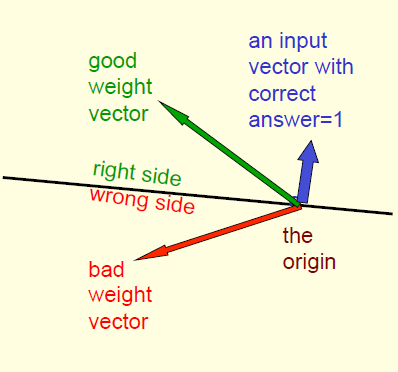
\includegraphics[scale=0.8]{wightspace.png}
\end{center}
If we have enough features and can choose them by hand, we can do almost anything. But once the hand-coded features have been determined, there are very strong limitations on what a perceptron can learn.

\subsection{Learning the weights of a linear neuron}
\[y = \sum\limits_i w_ix_i = w^Tx\]
But sometimes the weight will get worse. We can define the error as the squared residuals summed over all training cases. Then differantiate to get error derivatives for weights.

\subsection{Learning the weights of a logistic output neuron}
\[z = b + \sum\limits_i x_iw_i\]
\[y = \frac{1}{1 + e^{-z}}\]
We can use the chain rule to get the derivatives needed for learning the weights of a logistic unit.
\[\frac{\partial E}{\partial w_i} = \sum\limits_n \frac{\partial y^n}{\partial w_i}\frac{\partial E}{\partial y^n} = -\sum\limits_n x_i^ny^n(1 - y^n)(t^n - y^n)\]

\section{Plans for Next Week}
\begin{enumerate}
  \item Learn lecture11 to lecture13 of  \textbf{CS231n}.
  \item Learn week4 and week5 of \textbf{Neural Networks for Machine Learning}.
\end{enumerate}

\end{document}
